\documentclass{article}

\usepackage[utf8]{inputenc}
\usepackage[brazil]{babel}

\title{Exercício 5: Kernel Density Estimation}
\author{Rúbia Reis Guerra \\ 2013031143}

\usepackage{Sweave}
\begin{document}
\Sconcordance{concordance:mykde.tex:mykde.Rnw:%
1 8 1 1 0 8 1 1 2 1 0 3 1 1 6 4 0 1 4 2 0 8 1 1 4 2 0 3 1 3 0 1 2 1 1 1 %
4 3 0 3 1 1 2 1 1 1 73 71 0 1 2 2 1 1 2 5 0 1 1 6 0 1 2 39 1}

\maketitle

\section{Classificador Bayesiano: Kernel Density Estimation}
Nesta atividade, foi proposta a amostragem de dados do dataset BreastCancer, seguida da divisão em conjuntos de teste e treino e classifiação bayesiana. Para obter as densidades de cada classe, foi utilizado um estimador de densidade por kernel (KDE).

\section{Implementação}
\subsection{Pacotes utilizados}
\begin{Schunk}
\begin{Sinput}
> rm(list=ls())
> library('MASS')
> library('mlbench')
> library('flexclust')
> mykde <- function(x, X, n, N, h)
+ {
+   return((1/(N*(sqrt(2*pi)*h)^n))*
+       sum(exp(-((dist2(t(x),X)^2)/((2*h)^2)))))
+ }
> ###########################
> # Auxiliares #
> tp <- c()
> fp <- c()
> fn <- c()
> prec <- c()
> rec <- c()
> f1 <- c()
> error <- c()
> mse <- c()
> sde <- c()
> ###########################
> # Parâmetros #
> niter <- 10 # Número de iterações
> ptrain <- 0.7 # % conjunto de treino
> ptest <- 1 - ptrain # % conjunto de teste
> h <- 0.25
\end{Sinput}
\end{Schunk}

\subsection{Treinamento e Teste}
\begin{Schunk}
\begin{Sinput}
> ###########################
> # Dataset BreastCancer #
> data(BreastCancer)
> X <- data.matrix(BreastCancer[,2:10])
> X[is.na(X)] <- 0
> Y <- as.numeric(BreastCancer$Class)
> N <- dim(X)[1]
> n <- dim(X)[2]
> for(j in 1:niter){
+   ###########################
+   # Amostrar dados #
+   index <- sample(2, nrow(BreastCancer), replace=TRUE, prob=c(ptrain,ptest))
+   
+   ###########################
+   # Conjunto de treinamento #
+   training <- X[which(index==1),]
+   trainingLabels <- as.matrix(Y[which(index==1)])
+   
+   ###########################
+   # Conjunto de teste #
+   test <- X[which(index==2),]
+   testLabels <- as.matrix(Y[which(index==2)])
+   
+   ###########################
+   # Probabilidades a priori #
+   pc1 <- length(Y[which(Y==1)])/(length(Y))
+   pc2 <- length(Y[which(Y==2)])/(length(Y))
+   
+   ###########################
+   # Treinamento, teste e classificação #
+   Ntest <- dim(test)[1]
+   Ntrain <- dim(training)[1]
+   trc1 <- training[which(trainingLabels==1),]
+   trc2 <- training[which(trainingLabels==2),]
+   testY <- c()
+   pxc1 <- c()
+   pxc2 <- c()
+   
+   p11 <- c()
+   p12 <- c()
+   p21 <- c()
+   p22 <- c()
+   Nc1 <-  dim(trc1)[1]
+   Nc2 <-  dim(trc2)[1]
+ 
+   for(i in 1:Nc1)
+   {
+     p11[i] <- mykde(trc1[i,],trc1,n,N,h)
+     p12[i] <- mykde(trc1[i,],trc2,n,N,h)
+   }
+ 
+   for(i in 1:Nc2)
+   {
+     p21[i] <- mykde(trc2[i,],trc1,n,N,h)
+     p22[i] <- mykde(trc2[i,],trc2,n,N,h)
+   }
+   
+   for(i in 1:Ntest)
+   {
+     pxc1[i] <- mykde(test[i,],trc1,n,Ntrain,h)
+     pxc2[i] <- mykde(test[i,],trc2,n,Ntrain,h)
+     testY[i] <- ifelse(pxc1[i]/pxc2[i] >= pc2/pc1, 1, 2)
+     error[i] <- (testY[i]-testLabels[i])^2
+   }
+   
+   # MSE e SD #
+   mse[j] <- mean(error)
+   sde[j] <- sd(error)
+   
+   # Matriz de confusao #
+   testCM <- table(testY,testLabels)
+   
+   # Precision, recall, F1 #
+   tp[j] <- sum((testY==1) & (testLabels==1)) # True positives
+   fp[j] <- sum((testY==1) & (testLabels==2)) # False positives
+   fn[j] <- sum((testY==2) & (testLabels==1)) # False negatives
+   prec[j] <- tp[j]/(tp[j] + fp[j]) # Precision
+   rec[j] <- tp[j]/(tp[j] + fn[j]) # Recall
+   f1[j] <- 2*prec[j]*rec[j]/(prec[j]+rec[j]) # F1 Score
+ }
> plot(p11,p12,col='red',xlim=c(0,2),ylim=c(0,2),xlab='px1',ylab='px2')
> par(new=T)
> plot(p21,p22,col='blue',xlim=c(0,2),ylim=c(0,2),xlab='px1',ylab='px2')
> mean(mse) # MSE
\end{Sinput}
\begin{Soutput}
[1] 0.04035158
\end{Soutput}
\begin{Sinput}
> mean(sde) # SD
\end{Sinput}
\begin{Soutput}
[1] 0.196267
\end{Soutput}
\end{Schunk}

Para diferentes valores de h, foi possível observar valores de MSE baixos ($< 5\%$). Porém, para $h < 0.2$, os valores de densidade medidas para a classe 2 se aproximam de zero, causando anomalias na etapa de classificação.

\begin{figure}
  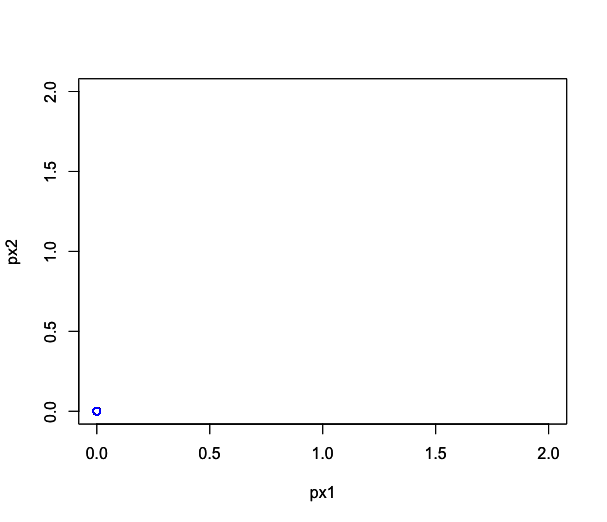
\includegraphics[width=\linewidth]{h08.png}
  \caption{h = 0.8, MSE = 0.046.}
  \label{fig:h08}
\end{figure}

\begin{figure}
  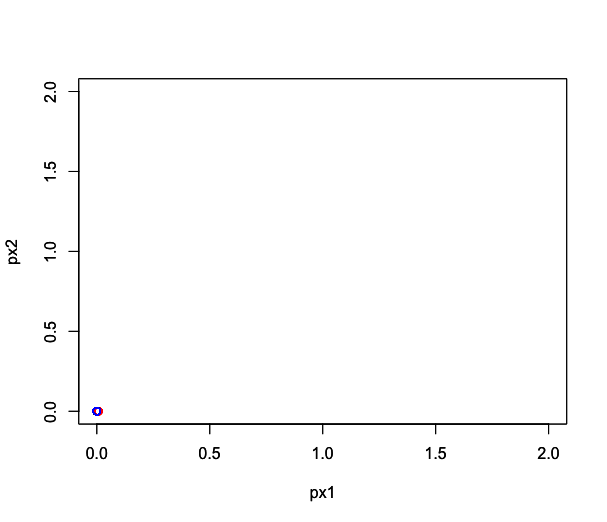
\includegraphics[width=\linewidth]{h05.png}
  \caption{h = 0.5, MSE = 0.044.}
  \label{fig:h05}
\end{figure}

\begin{figure}
  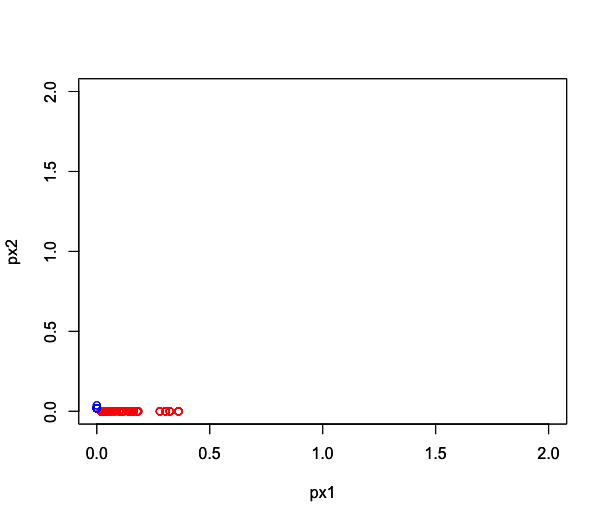
\includegraphics[width=\linewidth]{h03.png}
  \caption{h = 0.3, MSE = 0.039.}
  \label{fig:h03}
\end{figure}

\begin{figure}
  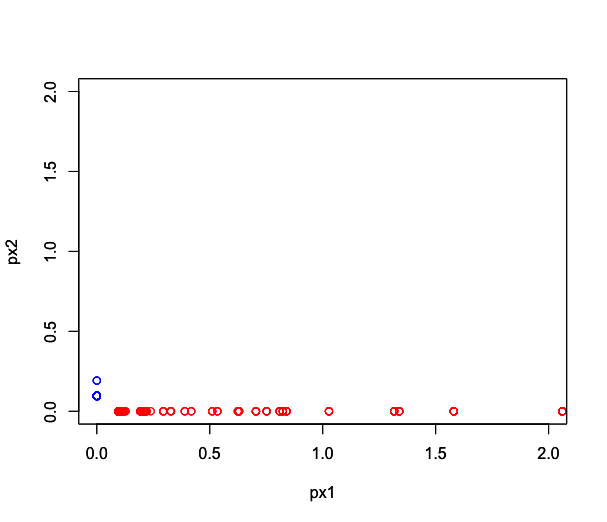
\includegraphics[width=\linewidth]{h025.png}
  \caption{h = 0.25, MSE = 0.048.}
  \label{fig:h025}
\end{figure}

\begin{figure}
  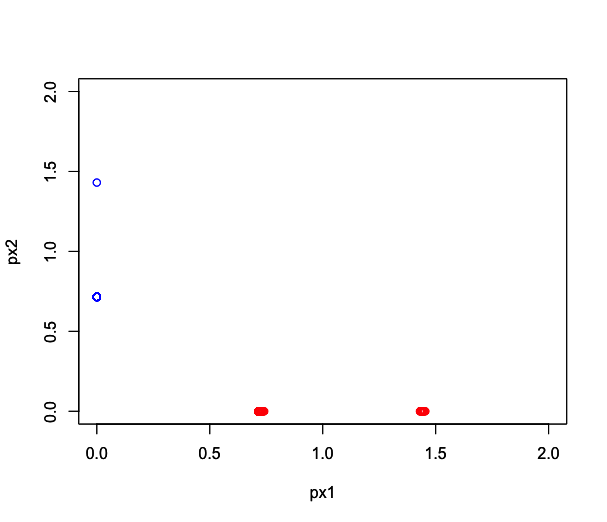
\includegraphics[width=\linewidth]{h02.png}
  \caption{h = 0.2, MSE = 0.043.}
  \label{fig:h02}
\end{figure}

\begin{figure}
  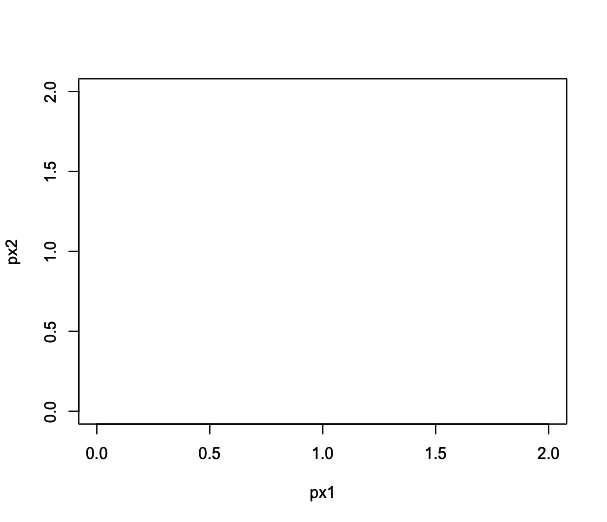
\includegraphics[width=\linewidth]{h015.png}
  \caption{h = 0.15, MSE = 0.00.}
  \label{fig:h015}
\end{figure}

\end{document}
